\section{译者补充:辐射度学、光度学与色度学}\label{sec:译者补充:辐射度学、光度学与色度学}

\begin{remark}
      本节内容不是原书内容,而是译者根据有关资料\citep{978-7-5640-0658-7,
            wiki:solidangle,GB3102.6-93,enwiki:1052681830,enwiki:SRGB,
            wiki:candela,Hoffmann2015,wiki:eye,BERTALMIO2020131}补充的,请酌情参考和斧正。
\end{remark}

\subsection{辐射度量}\label{sub:辐射度量}
立体角表示一个物体对特定点的三维空间角度,是平面角在三维空间中的类比。
它描述在某一点观测到的物体大小尺度。
例如对于一特定观察点,一个在该点附近的小物体
可能和一个远处的大物体有着相同的立体角。
\begin{definition}
      锥体的\keyindex{立体角}{solid angle}{}大小定义为:
      以锥体的顶点为球心作球面,该锥体在球表面截取的面积与球半径平方之比。
\end{definition}
立体角的单位为\keyindex{球面度}{steradian}{}(sr),是无量纲的导出单位。

\begin{figure}[htbp]
      \centering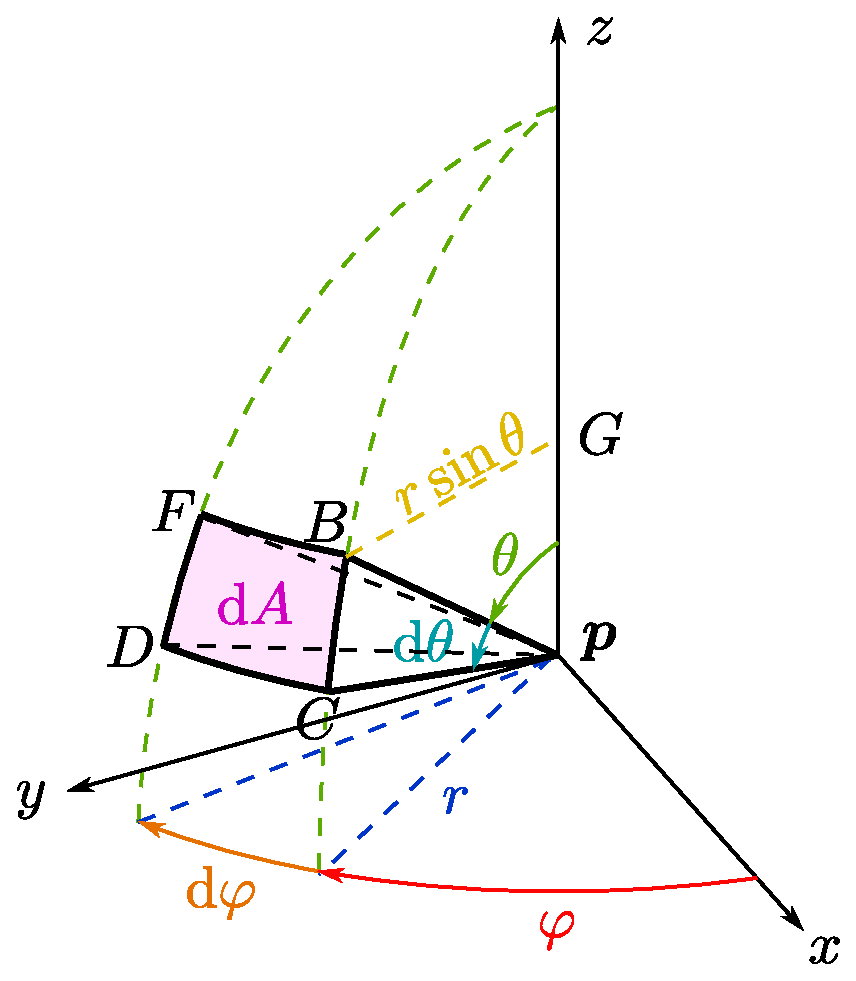
\includegraphics[width=0.4\linewidth]{chap05/ex-solidangle.eps}
      \caption{立体角的定义。}
      \label{fig:5.ex01}
\end{figure}

立体角常用字母$\varOmega$表示。\reffig{5.ex01}展示了一种简单的情形。
以$\bm p$为顶点的微分锥体${\bm p}-BCDF$在同样以$\bm p$为球心且半径为$r$的球面上截取下面元$BCDF$。
建立以$\bm p$为原点的球坐标系,则弧线$\wideparen{BC}$的\keyindex{方位角}{azimuth angle}{}
(在$xy$平面上的投影与原点连线和$x$正半轴所成角)为$\varphi$,
$\wideparen{DF}$方位角为$\varphi+\mathrm{d}\varphi$;
弧线$\wideparen{BF}$的\keyindex{天顶角}{zenith angle}{}(与原点连线和$z$正半轴所成角)为$\theta$,
$\wideparen{CD}$的天顶角为$\theta+\mathrm{d}\theta$。
因此点$B$到其在$z$轴投影点$G$的距离为$r\sin\theta$,
$\wideparen{BF}$的弧长为$r\sin\theta\mathrm{d}\varphi$;
同时$\wideparen{BC}$的弧长为$r\mathrm{d}\theta$。
将面元$BCDF$视作矩形,可求得其微分面积为
\begin{align}
      \mathrm{d}A=r\sin\theta\mathrm{d}\varphi\cdot r\mathrm{d}\theta\, .
\end{align}
依据定义,则相应的立体角元为
\begin{align}
      \mathrm{d}\varOmega=\frac{\mathrm{d}A}{r^2}=\sin\theta\mathrm{d}\theta\mathrm{d}\varphi\, .
\end{align}
对立体角元做曲面积分则可得立体角
\begin{align}
      \varOmega=\iint\limits_S \mathrm{d}\varOmega=\iint\limits_S \sin\theta\mathrm{d}\theta\mathrm{d}\varphi\, .
\end{align}

\begin{corollary}
      封闭曲面对于其内任意一点的立体角均为$4\pi$sr。
\end{corollary}

在连续意义下,我们定义以下辐射度量。

\begin{definition}
      \keyindex{辐射能}{radiant energy}{}指以电磁波形式发射、传播或接收的能量。
\end{definition}
辐射能常用$Q$表示,单位为\keyindex{焦耳}{joule}{}(焦,J)。

\begin{definition}
      \keyindex{辐射能通量}{radiant energy flux}{},
      也称\keyindex{辐射功率}{radiant power}{},
      指电磁辐射通过某一面积发射、传播或接收的功率。
\end{definition}
辐通量常用$\varPhi$表示,单位为\keyindex{瓦特}{watt}{}(瓦,W)。
它描述单位时间内的辐射能:
\begin{align}
      \varPhi=\frac{\mathrm{d}Q}{\mathrm{d}t}\, ,
\end{align}
其中$t$表示时间。

\begin{definition}
      \keyindex{辐射照度}{irradiance}{}/\keyindex{辐射出射度}{radiant exitance}{}指
      照射/离开表面一点处的单位面元上的辐射能通量。
\end{definition}
辐射照度常用$E$表示,辐射出射度常用$M$表示,单位均为$\text{W}/\text{m}^2$。
它们定义中面元所对应的立体角是辐射的整个半球空间,与辐通量的关系为
\begin{align}
      E(\text{或}M)=\frac{\mathrm{d}\varPhi}{\mathrm{d}A}\, ,
\end{align}
其中$A$为表面面积。

\begin{definition}
      \keyindex{辐射强度}{radiant intensity}{}指
      在给定方向的单位立体角元内离开点辐射源(或辐射源面元)的辐射通量。
\end{definition}
辐射强度常用$I$表示,单位为$\text{W}/\text{sr}$。
它一般适合于描述(近似)点光源的辐射方向特性,
与辐射通量和立体角的关系为
\begin{align}
      I=\frac{\mathrm{d}\varPhi}{\mathrm{d}\varOmega}\, .
\end{align}

\begin{definition}
      \keyindex{辐射亮度}{radiance}{}指
      表面一点在垂直于给定方向的单位面元上于该方向的辐射强度。
\end{definition}
辐射亮度常用$L$表示,单位为W$/$(sr$\cdot$m$^2$)。
它与其他辐射度量的关系为
\begin{align}\label{eq:5.ex-radiance}
      L=\frac{\mathrm{d}I}{\cos\theta\mathrm{d}A}=\frac{\mathrm{d}^2\varPhi}{\cos\theta\mathrm{d}A\mathrm{d}\varOmega}=\frac{\mathrm{d}E}{\cos\theta\mathrm{d}\varOmega}\, ,
\end{align}
其中$\theta$是曲面法线与给定方向的夹角。

\reffig{5.ex02}展示了辐射度量之间的微分关系。
\begin{figure}[htbp]
      \centering
      \begin{picture}(370,50)
            \put(0,0){辐射能$Q$}
            \put(45,3){\vector(1,0){40}}
            \put(50,6){时间$t$}
            \put(90,0){辐射通量$\varPhi$}
            \put(150,3){\vector(1,0){50}}
            \put(152,6){立体角$\varOmega$}
            \put(205,0){辐射强度$I$}
            \put(260,3){\vector(1,0){50}}
            \put(262,6){投影面积}
            \put(315,0){辐射亮度$L$}
            \put(120,12){\line(0,1){25}}
            \put(120,37){\vector(1,0){80}}
            \put(152,40){面积$A$}
            \put(205,35){辐射照度$E$}
            \put(260,37){\line(1,0){80}}
            \put(340,37){\vector(0,-1){25}}
            \put(262,40){余弦加权立体角}
      \end{picture}
      \caption{辐射度量的微分关系。}
      \label{fig:5.ex02}
\end{figure}

\subsection{光度学}\label{sub:光度学}
光度量是光辐射能为平均人眼接收所引起的视觉刺激大小的度量。
光度量和辐射度量的定义是一一对应的,都可以用来定量描述辐射的大小。
辐射度量是辐射能本身的客观度量,是纯粹的物理量;
而光度量则还考虑了生理学、心理学等因素。

\keyindex{发光强度}{luminous intensity}{}与辐射强度对应,
单位为坎德拉。
\begin{definition}
      频率为$540\times10^{12}\text{Hz}$(对应空气中555nm的波长)的单色辐射光源
      在给定方向上辐射强度为$\displaystyle\frac{1}{683}$W$/$sr时,
      其发光强度为1\keyindex{坎德拉}{candela}{}(cd)。
\end{definition}
坎德拉是国际单位制七个基本单位之一。
一只普通蜡烛的发光强度约为1cd。

\keyindex{光通量}{luminous flux}{}与辐射通量对应,
单位为\keyindex{流明}{lumen}{}(lm),1lm$=$1cd$\cdot$sr。

\begin{notation}
      我们约定后文光度量和对应的辐射度量所用字母相同,作区分时两者分别添加下标$\mathrm{v}$和$\mathrm{e}$。
      例如辐射强度记为$I_{\mathrm{e}}$,发光强度记为$I_{\mathrm{v}}$。
\end{notation}

\begin{notation}
      某一量的光谱密集度通常表示为波长(或频率)的函数,它具有该量除以波长的量纲,
      有时也称分布函数,为了简便也可用形容词“光谱(的)”代替“光谱密集度”。
      后文中我们约定这类量用下标$\lambda$标记。
      例如“辐射能通量的光谱密集度”可简称为“光谱辐射能通量”,记为$\varPhi_{\lambda}$,
      与辐射能通量$\varPhi$的关系是$\displaystyle\varPhi=\int \varPhi_{\lambda}\mathrm{d}\lambda$。
      但应注意到形容词“光谱(的)”也可用来表示某个量是波长(或频率)的函数,
      这类量的记号把$\lambda$写在圆括号内。
\end{notation}

人感知到的光的强弱与光的频率(波长)有关,这是人眼视觉系统特性决定的。
例如在辐射功率一定时,人眼会感觉黄绿光比红光和蓝光看起来更明亮。
为了描述光源发出可见光的能力,我们引入新的指标。

\begin{definition}
      \keyindex{光视效能}{luminous efficacy}{}是
      目视引起刺激的光通量与光源发出的辐射通量之比,
      记作$K$,单位为lm$/$W:
      \begin{align}
            K=\frac{\varPhi_{\mathrm{v}}}{\varPhi_{\mathrm{e}}}\, .
      \end{align}
\end{definition}

\reftab{5.ex01}列出了常见光源的光视效能。
\begin{table}[htbp]
      \centering
      \begin{tabular}{lc|lc}
            \toprule
            \textbf{光源类型} & \textbf{光视效能(lm$/$W)} & \textbf{光源类型} & \textbf{光视效能(lm$/$W)} \\
            \midrule
            钨丝灯(真空)    & 8.0 - 9.2                 & 日光灯            & 27 - 41                   \\
            钨丝灯(充气)    & 9.2 - 21.0                & 高压水银灯        & 34 - 45                   \\
            石英卤钨灯        & 30                        & 超高压水银灯      & 40.0 - 47.5               \\
            气体放电管        & 16 - 30                   & 钠光灯            & 60                        \\
            \bottomrule
      \end{tabular}
      \caption{常见光源的光视效能。}
      \label{tab:5.ex01}
\end{table}

\begin{definition}
      \keyindex{光谱光视效能}{spectral luminous efficacy}{luminous efficacy光视效能}记作$K(\lambda)$,是光视效能关于波长的函数,即
      \begin{align}
            K(\lambda)=\frac{\varPhi_{\mathrm{v}\lambda}}{\varPhi_{\mathrm{e}\lambda}}\, .
      \end{align}
\end{definition}

\begin{definition}
      $K(\lambda)$的最大值称为\keyindex{最大光谱光视效能}{maximum spectral luminous efficacy}{luminous efficacy光视效能},
      记作$K_{\mathrm{m}}$。它在频率为$540\times10^{12}\text{Hz}$时取得,值为683lm$/$W。
\end{definition}
这也是坎德拉的定义以该频率为标准的原因。

\begin{definition}
      \keyindex{光视效率}{luminous efficiency}{}记作$V$,定义为光视效能与最大光谱光视效能的比值,量纲为1:
      \begin{align}
            V=\frac{K}{K_{\mathrm{m}}}\, .
      \end{align}
\end{definition}

\begin{definition}
      \keyindex{光谱光视效率}{spectral luminous efficiency}{}函数,
      即光视效率关于波长的函数,也称\keyindex{光度函数}{luminosity function}{}、
      相对\keyindex{视见函数}{visual sensitivity function}{}等,记作$V(\lambda)$:
      \begin{align}
            V(\lambda)=\frac{K(\lambda)}{K_{\mathrm{m}}}\, .
      \end{align}
      它表征了人眼对各波长单色光的视觉灵敏度。
\end{definition}

因为人眼在不同亮度环境下的视觉灵敏度不同,所以$V(\lambda)$
分为\keyindex{明视觉}{photopic}{}和\keyindex{暗视觉}{scotopic}{}两种常用版本(\reffig{5.ex03})。
1971年国际照明委员会公布的明视觉的$V(\lambda)$标准值已于1972年由国际计量委员会批准。
\begin{figure}[htbp]
      \centering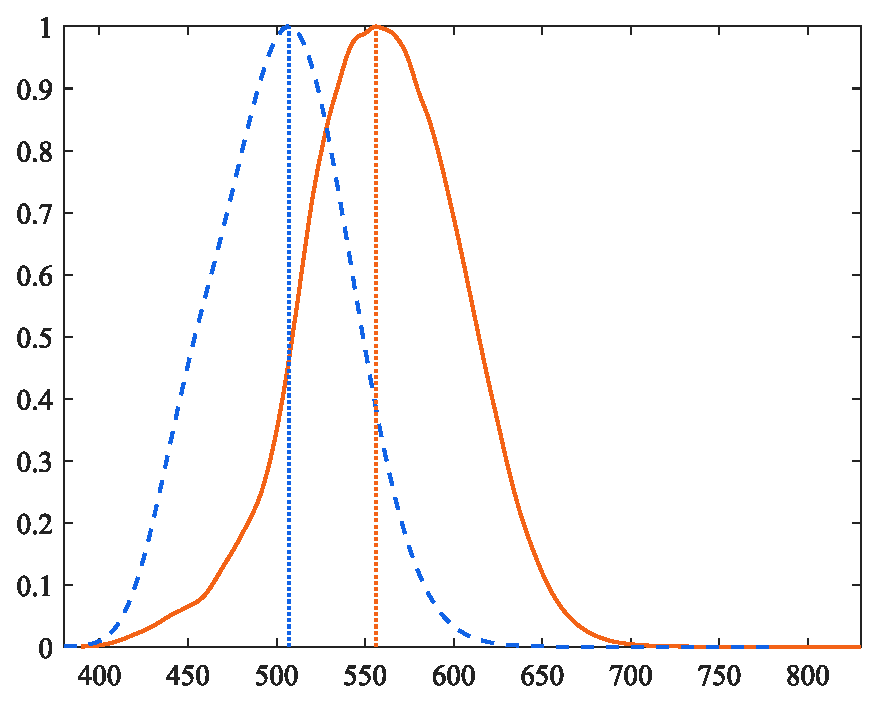
\includegraphics[width=0.75\linewidth]{chap05/spectralluminousefficiency.eps}
      \put(0,0){$\lambda/$nm}
      \put(-315,110){$V(\lambda)$}
      \caption{光谱光视效率曲线。其中橙色实线对应明视觉($2^{\circ}$视场角),蓝色虚线对应暗视觉。
            数据来源于\protect\url{http://www.cvrl.org}。}
      \label{fig:5.ex03}
\end{figure}

依据以上定义,可以推导出如下关系:
\begin{align}
      K                    & =\frac{\displaystyle\int \varPhi_{\mathrm{v}\lambda}\mathrm{d}\lambda}{\displaystyle\int \varPhi_{\mathrm{e}\lambda}\mathrm{d}\lambda}=\frac{\displaystyle\int K(\lambda)\varPhi_{\mathrm{e}\lambda}\mathrm{d}\lambda}{\displaystyle\int \varPhi_{\mathrm{e}\lambda}\mathrm{d}\lambda}\, , \\
      \varPhi_{\mathrm{v}} & =\displaystyle\int K(\lambda)\varPhi_{\mathrm{e}\lambda}\mathrm{d}\lambda=K_{\mathrm{m}}\int V(\lambda)\varPhi_{\mathrm{e}\lambda}\mathrm{d}\lambda\, ,                                                                                                                                    \\
      V                    & =\frac{\displaystyle\int V(\lambda)\varPhi_{\mathrm{e}\lambda}\mathrm{d}\lambda}{\displaystyle\int \varPhi_{\mathrm{e}\lambda}\mathrm{d}\lambda}\, .
\end{align}

\keyindex{光照度}{illuminance}{}与辐射照度对应,
\keyindex{光出射度}{luminous exitance}{}与辐射出射度对应,
单位均为\keyindex{勒克斯}{lux}{}(lx),1lx=1lm$/$m$^2$。

\keyindex{光亮度}{luminance}{}与辐射亮度对应,单位为cd$/$m$^2$。

\subsection{色度学}\label{sub:色度学}
\keyindex{色度学}{colorimetry}{}是在物理上量化描述人类颜色知觉的科学技术。
\subsubsection*{人眼视觉特性与颜色视觉理论}
人眼(\reffig{5.ex04})中负责感光的部分是\keyindex{视网膜}{retina}{},
其中具有两种\keyindex{感光细胞}{photoreceptor cell}{},
即\keyindex{视杆细胞}{rod cell}{}和\keyindex{视锥细胞}{cone cell}{}。
视杆细胞主要分布在视网膜中心周围,几乎全部用于夜视力,数量达到一亿量级。
1个光子就足以激发视杆细胞的活动,其对单个光子的敏感程度是视锥细胞的一百多倍,
因此视杆细胞建立人类在夜晚最基本的视觉,即暗视觉。
暗视觉只有视杆细胞起作用,由其仅含的视紫红色素吸收光子,所以不能分辨颜色,只有明暗感觉。
视锥细胞大多分布在视网膜黄斑处,因树突呈锥形得名,约有六百万个。
它主要负责颜色识别,在相对较亮的光照条件下发挥作用(一般需要数十到上百个光子激发),
按所含有的视色素分为三种,分别对黄绿色、绿色和蓝紫色的光最为敏感(\reffig{5.ex05}),
其形成的视觉信号复合后呈现出色彩缤纷的世界。
\begin{figure}[htbp]
      \centering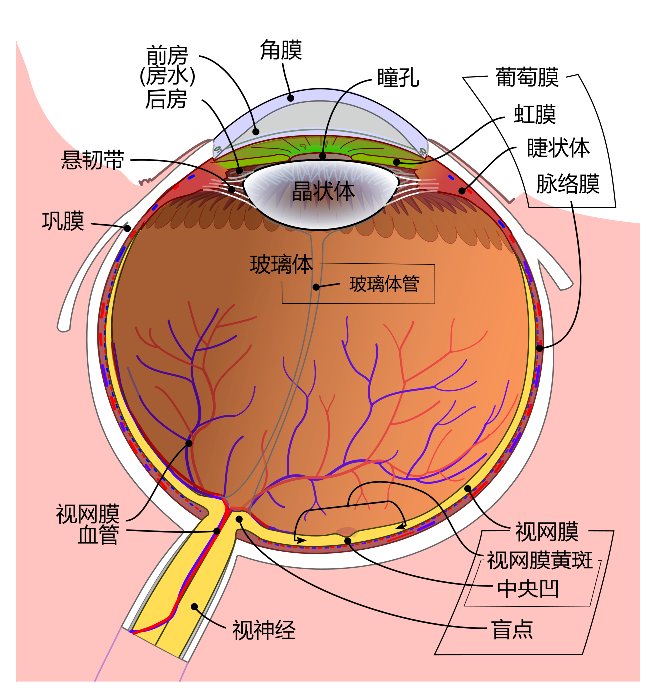
\includegraphics[width=0.5\linewidth]{chap05/Schematic_diagram_of_the_human_eye_zh-hans.eps}
      \caption{人眼结构。}
      \label{fig:5.ex04}
\end{figure}

\begin{figure}[htbp]
      \centering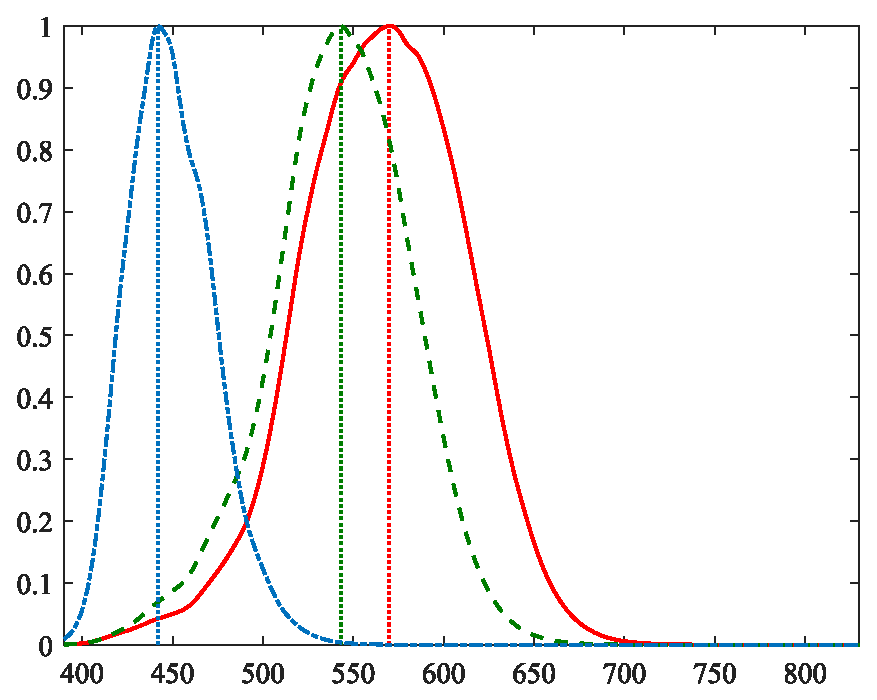
\includegraphics[width=0.75\linewidth]{chap05/NormalizedResponsivitySpectra.eps}
      \put(0,0){$\lambda/$nm}
      \put(-300,35){\rotatebox{90}{规范化视锥响应度(线性能量)}}
      \caption{人眼三种视锥细胞的规范化响应光谱($2^{\circ}$)。
            蓝、绿、红曲线分别对应S、M、L型视锥细胞。
            注意它们的响应绝对峰值并不相同,图中是规范化到0-1后的结果。
            数据来源于\protect\url{http://www.cvrl.org}。}
      \label{fig:5.ex05}
\end{figure}

现代颜色视觉理论主要有两大类,分别从是Yang-Helmholtz的三色学说和Hering的“对立”颜色学说发展起来的。
两者学说都能解释大量事实,但也都有不足之处。
三色学说能很好地说明各种颜色的混合现象,但不能很好地解释色盲现象;“对立”颜色学说则相反。
也有学者试图调和两者的观点。

\subsubsection*{颜色匹配}
\keyindex{颜色混合}{color mixing}{}可以是颜色光的混合,也可以是染料的混合,两种混合方法的结果是不同的,
前者称为\keyindex{加色混合}{additive mixing}{color mixing颜色混合},
后者称为\keyindex{减色混合}{subtractive mixing}{color mixing颜色混合}(\reffig{5.ex06})。
\begin{figure}[htb]
      \centering
      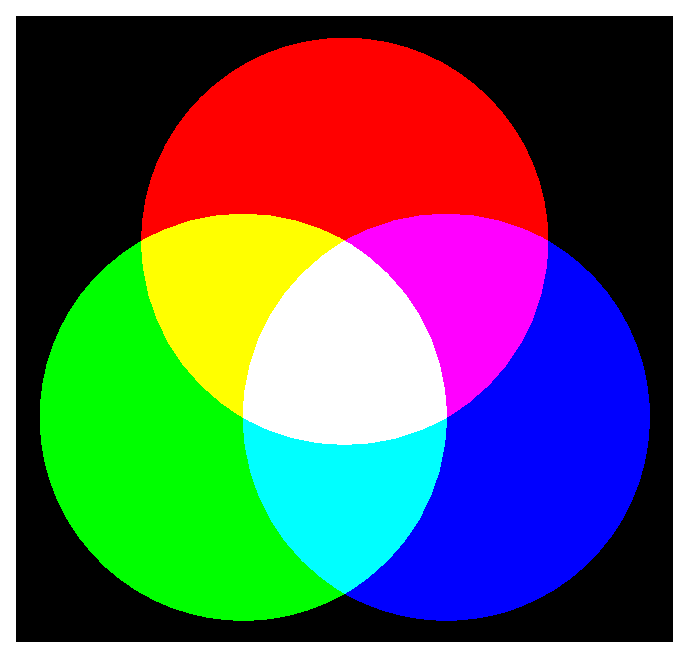
\includegraphics[width=0.4\linewidth]{chap05/additivemixing.eps}
      
\includegraphics[width=0.4\linewidth]{chap05/subtractivemixing.eps}
      \caption{颜色混合:加色混合(左)与减色混合(右)。}
      \label{fig:5.ex06}
\end{figure}

1853年,德国学者格拉斯曼(Hermann Günther Gra{\ss}mann)总结出加色混合的性质,
即格拉斯曼定律,为现代色度学奠定了基础。

\begin{proposition}
      \keyindex{格拉斯曼定律}{Grassmann's laws}{}的现代解释有四点内容:
      \begin{enumerate}
            \item 人的视觉只能分辨颜色的三种变化(例如明度、色调、饱和度)。
            \item 在由两种成分组成的混合色光中,若一种成分连续变化,则混合色光外观也连续变化。
            \item 存在光谱功率分布不同但外观相同的色光。
            \item 混合色光的总亮度是各成分亮度之和。
      \end{enumerate}
\end{proposition}
\begin{corollary}
      每种色光都存在\keyindex{互补色}{complementary color}{},
      使得两者混合后要么产生无色(白或灰)光,要么产生近似比重大的颜色成分的非饱和色。
\end{corollary}
\begin{corollary}
      任意两种非互补色混合会产生中间色,其色调和饱和度决定于两种成分的色调与相对数量。
\end{corollary}
\begin{corollary}
      若两种色光的外观相同,则它们在加色或减色混合中作成分时的效应是等价的。
\end{corollary}

例如若有两对颜色外观相同,即$A\equiv B$,$C\equiv D$,则有
\begin{align}
      A+C      & \equiv B+D\, ,      \\
      A-C      & \equiv B-D\, ,      \\
      \alpha A & \equiv \alpha B\, ,
\end{align}
其中符号“$\equiv$”表示颜色互相匹配。
即加色、减色混合的外观相同,颜色同时扩大或缩小相同倍数$\alpha>0$的外观相同。
这揭示了颜色混合的线性性质。

\begin{figure}[htbp]
      \centering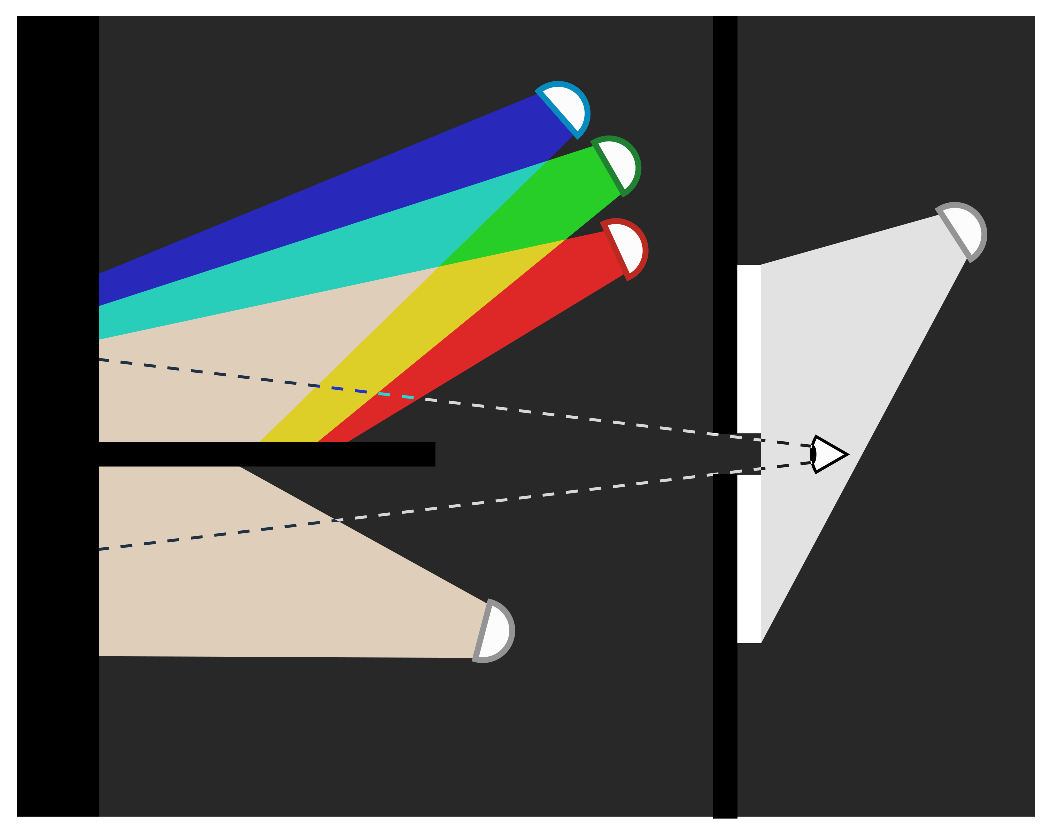
\includegraphics[width=0.75\linewidth]{chap05/colormatching.eps}
      \put(-120,195){\color[RGB]{6,139,190}蓝}
      \put(-105,178){\color[RGB]{31,129,49}绿}
      \put(-105,153){\color[RGB]{187,42,33}红}
      \put(-180,30){\color[RGB]{222,206,186}待匹配颜色光}
      \put(-155,95){\color{white}黑挡片}
      \put(-40,95){\color{white}眼}
      \put(-50,170){\color{white}背景光}
      \caption{颜色匹配实验。}
      \label{fig:5.ex07}
\end{figure}

结合来自1928年莱特(W. David Wright)、1931年吉尔德(John Guild)
以及1931年国际照明委员会(CIE)的颜色匹配实验数据,
CIE提出了“CIE 1931标准色度系统”。它们的实验方法都如\reffig{5.ex07}所示。
左边是一块白色屏幕,上方为红、绿、蓝三原色光,下方为待测色光。
三原色光照射白色屏幕的上半部分,待测色光照射下半部分,中间用黑挡片隔开。
从白色屏幕反射出来的光通过小孔抵达观察者人眼,视场为$2^{\circ}$并被分为两部分。
此外右上方还有一束颜色和强度可调的光照射在小孔周围的背景白板上。
在实验中,调节红、绿、蓝三原色光,直到观察者认为与待测色光的外观相同,
即视场中分界线感觉消失,两部分合为整体,
此时即三原混合色光与待测色光达到\keyindex{颜色匹配}{color matching}{}。
达到匹配后,改变背景光,此时视场中的颜色会变化,但仍能匹配。
颜色匹配时所需三原色的数量称为\keyindex{三刺激值}{tristimulus values}{}。
若分别以$\compcolor{C},\compcolor{R},\compcolor{G},\compcolor{B}$表示
被匹配的颜色以及红、绿、蓝三原色光的单位,以实数$C,R,G,B$表示相应颜色的数量,
则颜色匹配方程可写作
\begin{align}\label{eq:colormatchrgb}
      C\compcolor{C}\equiv R\compcolor{R}+G\compcolor{G}+B\compcolor{B}\, ,
\end{align}
其中符号“$\equiv$”表示颜色外观相同,$R,G,B$可以为负,$C=R+G+B$。

实验还证明了颜色匹配恒常律,即互相匹配的颜色在观察环境变化后依然保持匹配。
实验中在相应规定条件下视场为$2^{\circ}$的观察者
称为\keyindex{CIE 1931标准色度观察者}{CIE 1931 standard colorimetric observer}{}。

颜色匹配实验中有个重要问题是:以什么样的颜色作为三原色光?
三刺激值的单位$\compcolor{R},\compcolor{G},\compcolor{B}$如何确定?
原则上,三原色可以任意选定,但其中任何一种颜色不能由其他两种加色混合得到,最常用的是红、绿、蓝。
CIE在实验中使用波长分别为700nm、546.1nm、435.8nm的\keyindex{单色光}{monochromatic light}{}作为三原色,
其中700nm是可见光谱的红色末端,546.1nm和435.8nm是明显的汞谱线,三者在实验中都能比较精确地产生。
为了确定单位,CIE规定能匹配\keyindex{等能白光}{equal-energy white}{}(
也称\keyindex{E光源}{illuminant E}{},即整个光谱功率分布为常数的混合光,
因颜色接近白色得名,是一种理论光源,现实中暂无法模拟出来)且使得三刺激值全等
(即$R=G=B$)的三原色比例作为相应的色度学单位。
结果是,红绿蓝按光亮度之比为$1:4.5907:0.0601$
(对应于辐亮度之比$72.0962:1.3791:1$)作为三刺激值的单位。
\begin{example}
      按$0.1\compcolor{R}+0.2\compcolor{G}+0.3\compcolor{B}$所得的色光
      指按$(0.1\times1):(0.2\times4.5907):(0.3\times0.0601)=0.1:0.91814:0.01803$的
      光亮度比例混合波长分别700nm、546.1nm、435.8nm的单色光所得的结果。
\end{example}

实验中还发现,有一些颜色无论如何也无法被三原色匹配出来。
此时将某些三原色挪到与待测色光的同一侧进行实验则能实现匹配。
例如将红光与待测色光放在一侧,绿和蓝色光放在另一侧,当达到匹配时有
\begin{align}
      C\compcolor{C}+R'\compcolor{R}\equiv G\compcolor{G}+B\compcolor{B}\, .
\end{align}
于是可视作
\begin{align}
      C\compcolor{C}\equiv -R'\compcolor{R}+G\compcolor{G}+B\compcolor{B}\, ,
\end{align}
即三刺激值的红色分量为负值$-R'$。

单个波长的可见光称为\keyindex{光谱色}{spectral color}{}。
CIE依据历史与实验测定了匹配等能光谱色的RGB三刺激值,规范化后%规范化的具体做法未查到资料
得到RGB的\keyindex{颜色匹配函数}{color matching functions}{color matching颜色匹配},
记作$\bar{r}(\lambda),\bar{g}(\lambda),\bar{b}(\lambda)$,
并对应构建了\keyindex{CIE 1931 RGB 颜色空间}{CIE 1931 RGB color space}{}。
\reffig{5.ex08}显示$\bar{r}(\lambda)$在一定波长范围内取负值。
\begin{figure}[htbp]
      \centering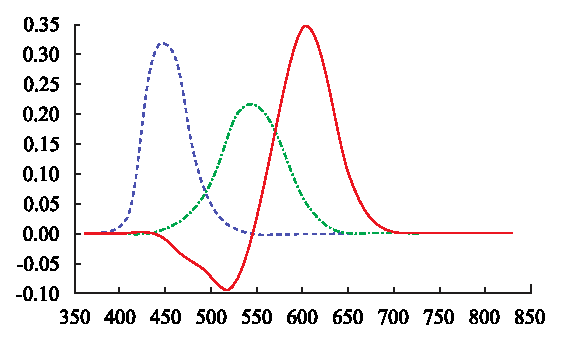
\includegraphics[width=0.75\linewidth]{chap05/CIERGBcolormatchingfunctions.eps}
      \put(10,0){$\lambda/$nm}
      \put(-110,125){$\bar{r}(\lambda)$}
      \put(-170,125){$\bar{g}(\lambda)$}
      \put(-235,125){$\bar{b}(\lambda)$}
      \caption{CIE RGB颜色匹配函数($2^{\circ}$视场),图示来自\citet{SETCHELL2012219}。}
      \label{fig:5.ex08}
\end{figure}

对于光谱分布为$S(\lambda)$的光刺激,相应的RGB值通过在颜色匹配函数上积分算得:
\begin{align}
      R & =k\int \bar{r}(\lambda)S(\lambda)\mathrm{d}\lambda\, , \\
      G & =k\int \bar{g}(\lambda)S(\lambda)\mathrm{d}\lambda\, , \\
      B & =k\int \bar{b}(\lambda)S(\lambda)\mathrm{d}\lambda\, ,
\end{align}
其中$k$为适当的规范化系数。

\subsubsection*{CIE 1931颜色空间}
\begin{definition}
      对于RGB三刺激值为$R,G,B$的颜色,定义其RGB\keyindex{色品}{chromaticity}{}坐标为:
      \begin{align}
            r & =\frac{R}{R+G+B}\, , \\
            g & =\frac{G}{R+G+B}\, , \\
            b & =\frac{B}{R+G+B}\, .
      \end{align}
\end{definition}
\begin{corollary}\label{corollary:chromaticity}
      色品坐标之和恒为1,即$r+g+b=1$。
\end{corollary}
这意味着色品坐标中只有两个独立分量。

依据RGB颜色匹配函数$\bar{r}(\lambda),\bar{g}(\lambda),\bar{b}(\lambda)$计算
出光谱色的色品坐标$r,g,b$,并以其中的$r$为横坐标,$g$为纵坐标,
按波长顺序将光谱色的色品点连接起来,可以得到舌形的轨迹(\reffig{5.ex09}),
称为\keyindex{光谱轨迹}{spectral locus}{}。
该轨迹在CIE RGB三原色波长处与坐标轴相交\sidenote{请读者思考一下为什么。},
即在435.8nm处有$r=0,g=0$,在546.1nm处有$r=0,g=1$,在700nm处有$r=1,g=0$。
光谱轨迹及其首尾连线围成封闭区域,
即构成\keyindex{CIE 1931 RGB 颜色空间}{CIE 1931 RGB color space}{}
\sidenote{它包含了人眼可见的全部颜色。}。
注意与\reffig{5.ex08}结合起来思考波长较短的轨迹为何进入$r<0$的半平面。
\begin{figure}[htbp]
      \centering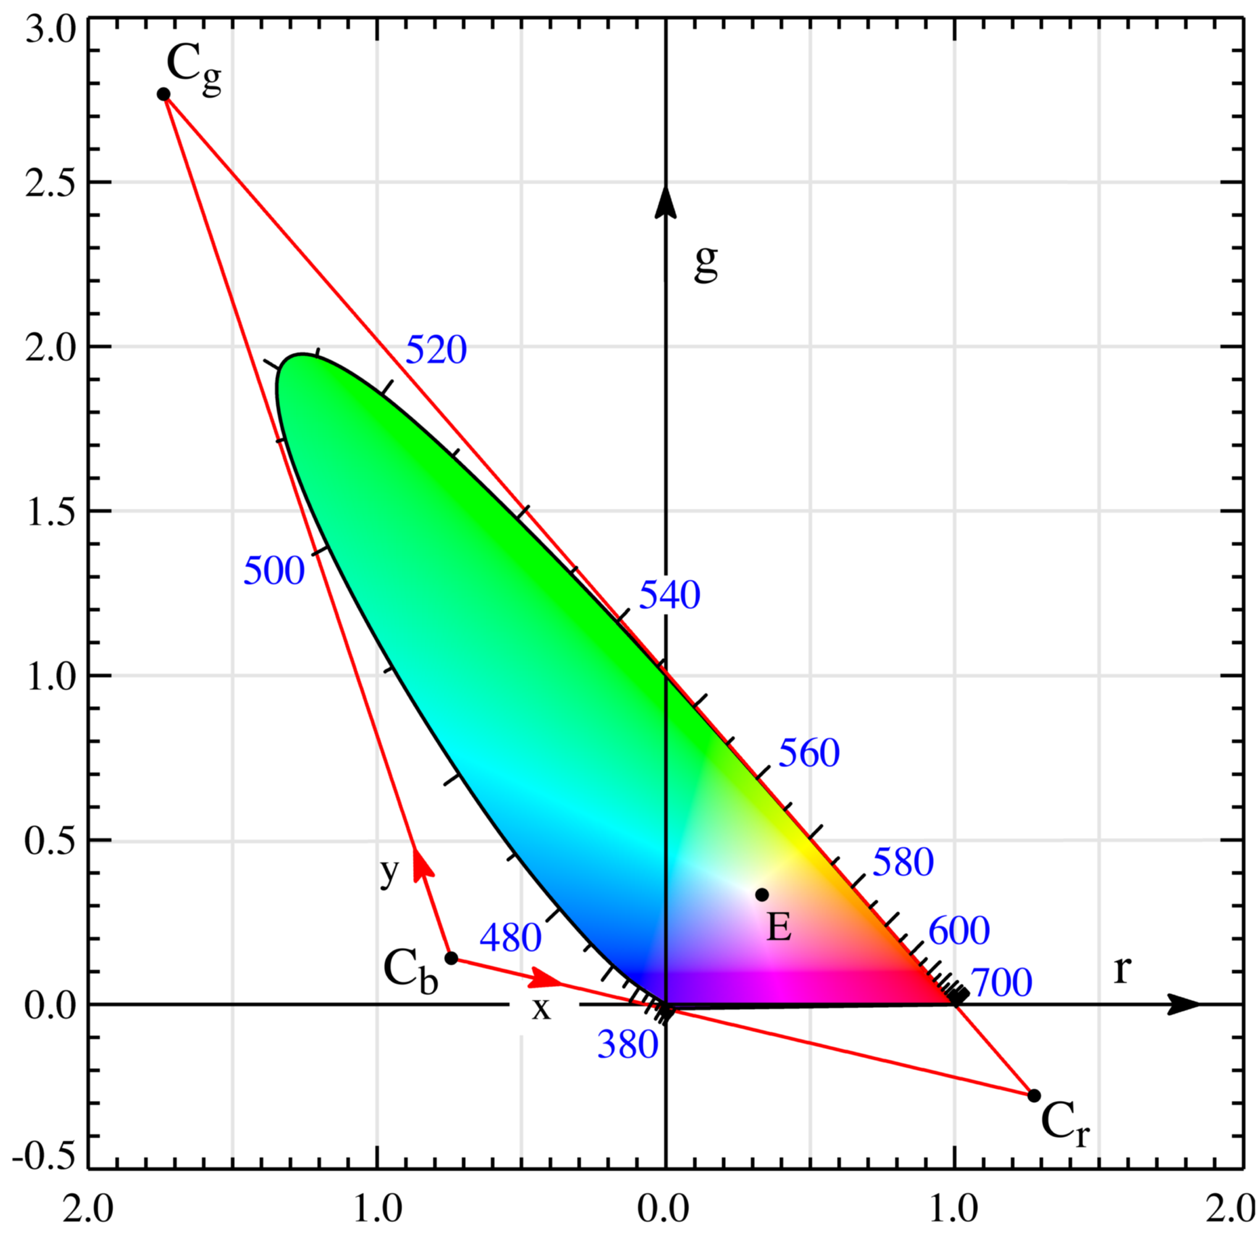
\includegraphics[width=0.75\linewidth]{chap05/CIE1931rgxy.png}
      \put(-205,9){\small -}
      \put(-270,9){\small -}
      \caption{CIE $rg$色品空间。其中E为等能白光;
      $\text{C}_{\mathrm{r}},\text{C}_{\mathrm{g}},\text{C}_{\mathrm{b}}$分别为
      $\compcolor{X},\compcolor{Y},\compcolor{Z}$三原色的色品点。
      $\text{C}_{\mathrm{r}}$与$\text{C}_{\mathrm{b}}$的连线为零亮度线。}
      \label{fig:5.ex09}
\end{figure}

依据颜色混合的线性性质,我们有:
\begin{corollary}
      对于由任意两种颜色$A,B$加色混合所得的颜色$C$,
      其色品点一定在$A$与$B$色品点所连的线段上。
\end{corollary}

虽然RGB颜色空间的$\bar{r}(\lambda),\bar{g}(\lambda),\bar{b}(\lambda)$
可用于色度计算,但其出现的负值不易理解且使用不便。
因此CIE定义了三种假想的三原色$\compcolor{X},\compcolor{Y},\compcolor{Z}$,
构建新的颜色空间以消除负值。其在构建过程中还考虑了以下问题:
\begin{enumerate}
      \item 规定$\compcolor{X}$和$\compcolor{Z}$只代表色度,与亮度无关。
            光亮度只与$\compcolor{Y}$的刺激值$Y$成正比。
            称$\compcolor{X}$和$\compcolor{Z}$在色品图中的连线为\keyindex{零亮度线}{alychne}{}。
            因为$\compcolor{R},\compcolor{G},\compcolor{B}$的光亮度之比为$1:4.5907:0.0601$,
            故零亮度线上的色品坐标应满足
            \begin{align}
                  r+4.5907g+0.0601b=0\, ,
            \end{align}
            代入$b=1-r-g$得
            \begin{align}
                  0.9399r+4.5306g+0.0601=0\, .
            \end{align}
      \item 所有光谱三刺激值均为非负数。因此$\compcolor{X},\compcolor{Y},\compcolor{Z}$所
            围成的三角形必须能包围整个光谱轨迹。
      \item $rg$色品图中光谱轨迹从540nm附近到700nm几乎是一条直线,
            这段线段上的任意两种颜色加色混合可匹配两色之间的各种光谱色。
            因此希望$\compcolor{X}$和$\compcolor{Y}$的连线与该线段重合,
            使其只与$\compcolor{X}$和$\compcolor{Y}$的变化有关,与$\compcolor{Z}$无关。
\end{enumerate}

此外$\compcolor{YZ}$边取光谱轨迹在波长503nm处的切线。
于是直线$\compcolor{XY}$、$\compcolor{YZ}$和$\compcolor{XZ}$均得以确定。
它们的交点即$\compcolor{X},\compcolor{Y},\compcolor{Z}$在$rg$色品图中的位置。
以$\compcolor{X},\compcolor{Y},\compcolor{Z}$为三原色的颜色空间
即\keyindex{CIE 1931 XYZ 颜色空间}{CIE 1931 XYZ color space}{}。
注意$\compcolor{X},\compcolor{Y},\compcolor{Z}$是现实中观察不到的理论假想色。
在该颜色空间中,颜色匹配方程为
\begin{align}\label{eq:colormatchxyz}
      C\compcolor{C}\equiv X\compcolor{X}+Y\compcolor{Y}+Z\compcolor{Z}\, .
\end{align}
其中$X,Y,Z$为相应的三刺激值。
依据构建过程中考虑的第1点问题,$Y$的光谱分布就是光谱光视效率函数,即
\begin{align}
      Y(\lambda)=V(\lambda)\, .
\end{align}
与$X,Y,Z$对应的XYZ色品坐标为
\begin{align}
      x & =\frac{X}{X+Y+Z}\, , \\
      y & =\frac{Y}{X+Y+Z}\, , \\
      z & =\frac{Z}{X+Y+Z}\, .
\end{align}
它同样满足推论\ref{corollary:chromaticity},即$x+y+z=1$。

与RGB类似,我们可以得到对应于光谱色的
CIE XYZ 颜色匹配函数$\bar{x}(\lambda),\bar{y}(\lambda),\bar{z}(\lambda)$(\reffig{5.ex10})
以及马蹄形的光谱轨迹与$xy$色品图(\reffig{5.ex11})。
可以看到$\bar{x}(\lambda),\bar{y}(\lambda),\bar{z}(\lambda)$不再含有负数,
光谱轨迹完全在$xy$第一象限。其中光谱轨迹的首尾连线称为\keyindex{紫线}{line of purples}{}。
\begin{figure}[htbp]
      \centering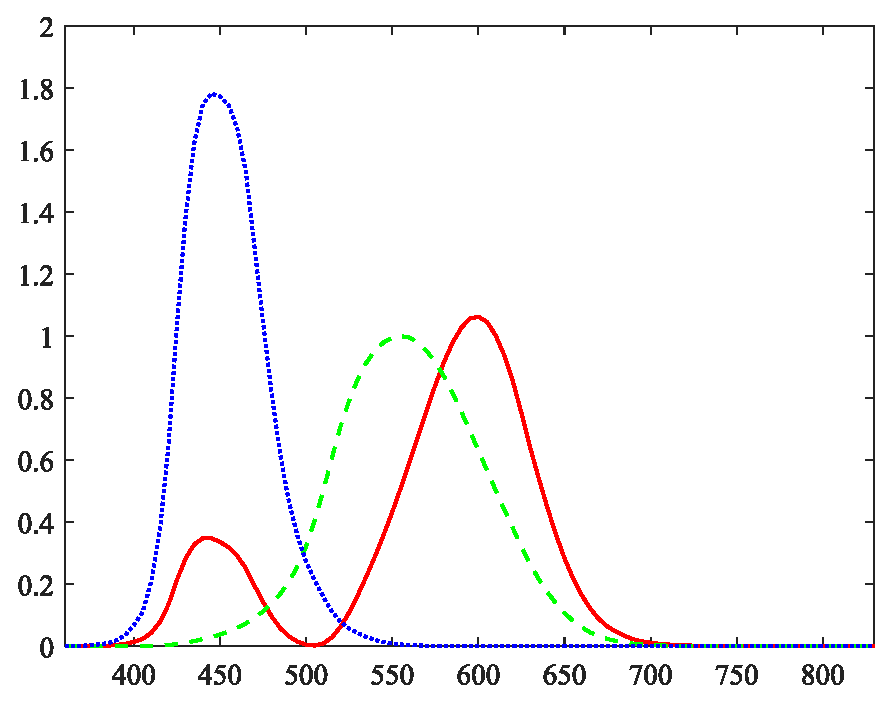
\includegraphics[width=0.75\linewidth]{chap05/cie31xyz.eps}
      \put(0,0){$\lambda/$nm}
      \put(-110,100){$\bar{x}(\lambda)$}
      \put(-170,125){$\bar{y}(\lambda)$}
      \put(-250,125){$\bar{z}(\lambda)$}
      \caption{CIE XYZ颜色匹配函数($2^{\circ}$视场),数据来源于\protect\url{http://www.cvrl.org}。}
      \label{fig:5.ex10}
\end{figure}

类似于RGB,对于光谱分布为$S(\lambda)$的光刺激,相应的XYZ值通过在颜色匹配函数上积分算得:
\begin{align}
      X & =k\int \bar{x}(\lambda)S(\lambda)\mathrm{d}\lambda\, , \\
      Y & =k\int \bar{y}(\lambda)S(\lambda)\mathrm{d}\lambda\, , \\
      Z & =k\int \bar{z}(\lambda)S(\lambda)\mathrm{d}\lambda\, ,
\end{align}
其中$k$为适当的规范化系数。

\begin{figure}[htbp]
      \centering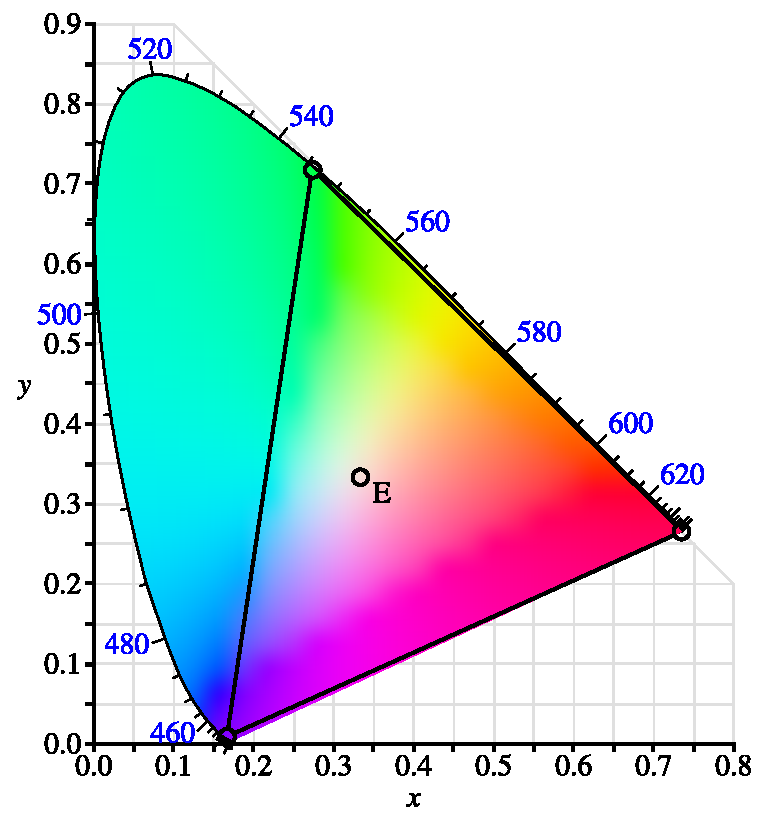
\includegraphics[width=0.6\linewidth]{chap05/CIE1931xyCIERGB.pdf}
      \caption{CIE 1931 XYZ颜色空间色品图。图中的三角形标出了CIE RGB三原色的位置。
            注意因为当下显示和打印设备的色域均不能覆盖整个颜色空间,加之图片格式的限制,
            所以该图中的一部分颜色一定会显示得不准确。}
      \label{fig:5.ex11}
\end{figure}

注意到当$X+Y+Z=1$时,有$x=X,y=Y,z=Z$。
这说明$xy$色品图是在$XYZ$坐标系中
截取平面$X+Y+Z=1$再向$XY$平面投影的结果(\reffig{5.ex12})。
\begin{figure}[htbp]
      \centering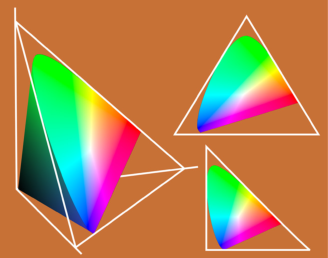
\includegraphics[width=0.5\linewidth]{chap05/Projectionandchromaticityplane.pdf}
      \put(-80,38){\color{white}$X$}
      \put(-165,130){\color{white}$Y$}
      \put(-160,4){\color{white}$Z$}
      \caption{XYZ体与$xy$色品图。左图是XYZ体,右上是截平面$X+Y+Z=1$,
            右下是将截平面投影到$XY$平面得到的$xy$色品图。图示来自\protect\citet{BERTALMIO2020131}。}
      \label{fig:5.ex12}
\end{figure}

\subsubsection*{颜色空间的转化}
由于选择的三原色以及三刺激值单位不同,出现了多种颜色空间。
这里我们介绍RGB与XYZ颜色空间相互转化的推导过程。

以XYZ转化到RGB空间为例。XYZ为旧空间,RGB为新空间。
设新空间的三原色$\compcolor{R},\compcolor{G},\compcolor{B}$在
旧空间中的三刺激值为$X_i,Y_i,Z_i,(i=\mathrm{r},\mathrm{g},\mathrm{b})$,即
\begin{align}\label{eq:colorbasis}
      \compcolor{R} & =X_\mathrm{r}\compcolor{X}+Y_\mathrm{r}\compcolor{Y}+Z_\mathrm{r}\compcolor{Z}\, , \\
      \compcolor{G} & =X_\mathrm{g}\compcolor{X}+Y_\mathrm{g}\compcolor{Y}+Z_\mathrm{g}\compcolor{Z}\, , \\
      \compcolor{B} & =X_\mathrm{b}\compcolor{X}+Y_\mathrm{b}\compcolor{Y}+Z_\mathrm{b}\compcolor{Z}\, .
\end{align}
对照颜色匹配方程\refeq{colormatchrgb}与\refeq{colormatchxyz},可得
\begin{align}
      X\compcolor{X}+Y\compcolor{Y}+Z\compcolor{Z}=R\compcolor{R}+G\compcolor{G}+B\compcolor{B}\, .
\end{align}
联立以上式子,由对应系数相等整理可得
\begin{align}
      \left[\begin{array}{c}
                  X \\Y\\Z
            \end{array}\right]=
      \left[\begin{array}{ccc}
                  X_\mathrm{r} & X_\mathrm{g} & X_\mathrm{b} \\
                  Y_\mathrm{r} & Y_\mathrm{g} & Y_\mathrm{b} \\
                  Z_\mathrm{r} & Z_\mathrm{g} & Z_\mathrm{b}
            \end{array}\right]
      \left[\begin{array}{c}
                  R \\G\\B
            \end{array}\right]\, .
\end{align}
上式表明两种颜色空间是线性转换关系,只要知道九个系数$X_i,Y_i,Z_i,(i=\mathrm{r},\mathrm{g},\mathrm{b})$即可。
实际中更常见的是这些系数待定,但知道对应的色品坐标$x_i,y_i,z_i,(i=\mathrm{r},\mathrm{g},\mathrm{b})$。设
\begin{align}
      C_i=X_i+Y_i+Z_i\, ,\quad (i=\mathrm{r},\mathrm{g},\mathrm{b})\, ,
\end{align}
则有
\begin{align}\quad
      X_i=C_ix_i\, ,\quad Y_i=C_iy_i\, ,\quad Z_i=C_iz_i\, ,\quad (i=\mathrm{r},\mathrm{g},\mathrm{b})\, .
\end{align}
记
\begin{align}
      P & =\left[\begin{array}{ccc}
                  x_\mathrm{r} & x_\mathrm{g} & x_\mathrm{b} \\
                  y_\mathrm{r} & y_\mathrm{g} & y_\mathrm{b} \\
                  z_\mathrm{r} & z_\mathrm{g} & z_\mathrm{b}
            \end{array}\right]\, , \\
      D & =\left[\begin{array}{ccc}
                  C_\mathrm{r} &              &              \\
                               & C_\mathrm{g} &              \\
                               &              & C_\mathrm{b}
            \end{array}\right]\, ,
\end{align}
于是
\begin{align}
      [X\quad Y\quad Z]^{\mathrm{T}}=PD[R\quad G\quad B]^{\mathrm{T}}\, .
\end{align}
其中矩阵$P$是已知的,还需确定$D$中的三个系数$C_i$,
一般我们通过选择一种颜色(例如参照白)
在旧空间的三刺激值$X_0,Y_0,Z_0$以及规定它在新空间的三刺激值$R_0,G_0,B_0$来求解,即
\begin{align}
      [X_0\quad Y_0\quad Z_0]^{\mathrm{T}}=PD[R_0\quad G_0\quad B_0]^{\mathrm{T}}\, .
\end{align}
可解得
\begin{align}
      \left[\begin{array}{c}
                  C_\mathrm{r} \\C_\mathrm{g}\\C_\mathrm{b}
            \end{array}\right]=\left(P
      \left[\begin{array}{ccc}
                  R_0 &     &     \\
                      & G_0 &     \\
                      &     & B_0
            \end{array}\right]\right)^{-1}
      \left[\begin{array}{c}
                  X_0 \\Y_0\\Z_0
            \end{array}\right]\, .
\end{align}
此时转化关系得以完全确定。还可得逆转化关系相应为
\begin{align}
      [R\quad G\quad B]^{\mathrm{T}}=(PD)^{-1}[X\quad Y\quad Z]^{\mathrm{T}}\, .
\end{align}

对于CIE 1931 RGB颜色空间与XYZ空间的转化,以等能白光为参照取
\begin{align}
      \begin{array}{lll}
            x_\mathrm{r}=0.73467\, , & x_\mathrm{g}=0.27376\, , & x_\mathrm{b}=0.16658\, , \\
            y_\mathrm{r}=0.26533\, , & y_\mathrm{g}=0.71741\, , & y_\mathrm{b}=0.00886\, , \\
            X_0=Y_0=Z_0=1\, ,        & R_0=G_0=B_0=1\, .        &
      \end{array}
\end{align}
算得
\begin{align}
      PD        & =\left[\begin{array}{rrr}
                  0.4900  & 0.3100 & 0.2000 \\
                  0.1770  & 0.8124 & 0.0106 \\
                  -0.0000 & 0.0100 & 0.9900
            \end{array}\right]\, , \\
      (PD)^{-1} & =\left[\begin{array}{rrr}
                  2.3647  & -0.8966 & -0.4681 \\
                  -0.5152 & 1.4264  & 0.0887  \\
                  0.0052  & -0.0144 & 1.0092
            \end{array}\right]\, .
\end{align}

\keyindex{sRGB颜色空间}{standard RGB color space}{}是惠普与微软等企业
于1996年共同开发的用于显示器、打印机以及互联网的一种色域标准。
对于sRGB的线性值与XYZ空间的转化,以D65为参照白\sidenote{D65是CIE规定的标准日光光源,色温约6500{\normalfont K}。}取
\begin{align}
      \begin{array}{lll}
            x_\mathrm{r}=0.6400\, , & x_\mathrm{g}=0.3000\, , & x_\mathrm{b}=0.1500\, , \\
            y_\mathrm{r}=0.3300\, , & y_\mathrm{g}=0.6000\, , & y_\mathrm{b}=0.0600\, , \\
            x_0=0.3127\, ,          & y_0=0.3290\, ,          & Y_0=1.0000\, ,          \\
            R_0=G_0=B_0=1\, .       &                         &
      \end{array}
\end{align}
算得
\begin{align}
      PD        & =\left[\begin{array}{rrr}
                  0.4124 & 0.3576 & 0.1805 \\
                  0.2126 & 0.7152 & 0.0722 \\
                  0.0193 & 0.1192 & 0.9505
            \end{array}\right]\, , \\
      (PD)^{-1} & =\left[\begin{array}{rrr}
                  3.2410  & -1.5374 & -0.4986 \\
                  -0.9692 & 1.8760  & 0.0416  \\
                  0.0556  & -0.2040 & 1.0570
            \end{array}\right]\, .
\end{align}

sRGB在完成RGB线性值(在0到1之间)的计算后,还要进行非线性的伽马校正才得到最终结果。
对于线性值$C(=R,G,B)$,相应最终值为
\begin{align}
      C_{\text{sRGB}}=\left\{
      \begin{array}{ll}
            \displaystyle12.92C\, ,                       & \text{若}C\le0.0031308\, , \\
            \displaystyle1.055C^{\frac{1}{2.4}}-0.055\, , & \text{其他}\, .
      \end{array}
      \right.
\end{align}
由最终值到线性值的逆变换为
\begin{align}
      C=\left\{
      \begin{array}{ll}
            \displaystyle\frac{C_{\text{sRGB}}}{12.92}\, ,                          & \text{若}C_{\text{sRGB}}\le0.04045\, , \\
            \displaystyle\left(\frac{C_{\text{sRGB}}+0.055}{1.055}\right)^{2.4}\, , & \text{其他}\, .
      \end{array}
      \right.
\end{align}

\reffig{5.ex13}展示了多种\keyindex{色域}{color gamut}{}标准。
\begin{figure}[htbp]
      \centering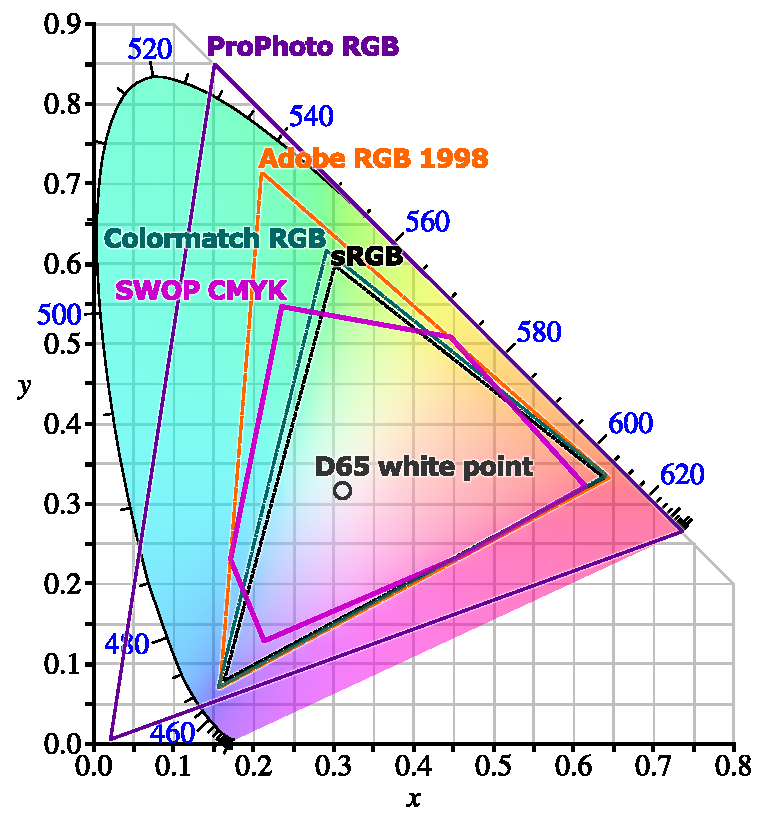
\includegraphics[width=0.6\linewidth]{chap05/CIE1931xygamutcomparison.pdf}
      \caption{一些RGB与CMYK色域在CIE 1931 $xy$色品图中的范围。}
      \label{fig:5.ex13}
\end{figure}